%!TeX root=./injoit-rus.tex

% Вставьте ссылки на файлы с текстом статьи
\newcommand*{\Source}{
    %!TeX root=../injoit-rus.tex

\section{Введение}
\label{sec:intro}
Душа моя озарена неземной радостью, как эти чудесные весенние утра, которыми я наслаждаюсь от всего сердца.
Я совсем один и блаженствую в здешнем краю, словно созданном для таких, как я.
Я так счастлив, мой друг, так упоен ощущением покоя, что искусство мое страдает от этого. Ни одного штриха не мог бы я сделать, а никогда не был таким большим художником, как в эти минуты.
Когда от милой моей долины поднимается пар и полдневное солнце стоит над непроницаемой чащей темного леса и лишь редкий луч проскальзывает в его святая святых, а я лежу в высокой траве у быстрого ручья и, прильнув к земле, вижу тысячи всевозможных былинок и чувствую, как близок моему сердцу крошечный мирок, что снует между стебельками, наблюдаю эти неисчислимые, непостижимые разновидности червяков и мошек и чувствую близость всемогущего, создавшего нас по своему подобию, веяние вселюбящего, судившего нам парить в вечном блаженстве, когда взор мой туманится и все вокруг меня и небо надо мной запечатлены в моей душе, точно образ возлюбленной,~--- тогда, дорогой друг, меня часто томит мысль: \textquote{Ах! Как бы выразить, как бы вдохнуть в рисунок то, что так полно, так трепетно живет во мне, запечатлеть отражение моей души, как душа моя~--- отражение предвечного бога!}

    %!TeX root=../injoit-rus.tex

\section{Связанные работы}
\label{sec:literature}
Методы обфускации и метаморфизма кода являются предметом исследований в области компьютерной безопасности и программной инженерии на протяжении нескольких десятилетий. Фундаментальные техники обфускации, такие как вставка неиспользуемого кода, модификация потока управления, переименование идентификаторов и преобразование данных, были систематизированы и подробно описаны в основополагающих работах, например, Collberg и др. \cite{Collberg97Survey}. Метаморфизм, как развитие идей обфускации, фокусируется на самомодификации кода с целью уклонения от обнаружения, что детально рассмотрено в работе Szor \cite{Szor05Metamorphic}. Различные аспекты эволюции и реализации метаморфических техник также анализируются в обзорах Sharma и Sahay \cite{Sharma14Evolution} и Brezinski и Ferens \cite{Brezinski21Survey}.

Несмотря на глубокую теоретическую проработку, автоматизация метаморфизма остается сложной задачей. Существующие инструментарии часто либо являются коммерческими продуктами с закрытым исходным кодом, либо представляют собой академические прототипы или генераторы вредоносного ПО, ориентированные на низкоуровневые представления кода (байт-код, ассемблер) и специфические платформы \cite{Brezinski21Survey}. Обзоры средств защиты программного обеспечения, такие как работа Schrittwieser и др. \cite{Schrittwieser16Survey}, часто отмечают ограничения существующих общедоступных инструментов обфускации, которые редко реализуют сложные метаморфические преобразования и не обладают адаптивностью. Большинство подходов либо применяют предопределенный набор правил, либо требуют значительного ручного вмешательства для настройки.

Исследования в области применения машинного обучения и формальных методов чаще фокусировались на обнаружении и анализе метаморфического кода \cite{Wong06Hunting, Campion21Learning}, а не на его автоматизированной генерации с целью защиты легитимного ПО. Подходы к изучению правил трансформации из образцов \cite{Campion21Learning} интересны, но не решают задачу создания метаморфического кода по запросу.

Данная работа направлена на восполнение этого пробела. В отличие от классических инструментов, мы предлагаем подход, использующий возможности современных LLM для автоматизации метаморфических преобразований непосредственно на уровне исходного кода языка Go. Мы не фокусируемся на низкоуровневых представлениях и не привязываемся к конкретным архитектурам, делегируя интеллектуальную часть генерации преобразований внешним моделям ИИ, что отличает наш подход от большинства существующих решений.

    \section{Методология и Инструментарий}

Для решения задачи автоматизации метаморфизма кода Go с использованием больших языковых моделей была разработана и реализована специализированная методология, воплощенная в программном инструментарии. Основой инструментария является модульная архитектура, реализованная на языке Go, что обеспечивает гибкость, производительность и удобство разработки. Проект структурирован с разделением на пользовательский интерфейс командной строки и внутреннюю логику преобразования кода.

Центральным компонентом системы является пакет \texttt{internal/rewriter}, инкапсулирующий всю логику, связанную с метаморфическими преобразованиями. Ключевая особенность данного модуля заключается в том, что он выступает в роли абстрактного интерфейса к внешним LLM, не реализуя самостоятельно алгоритмы обфускации. Его задача — получить фрагмент исходного Go-кода, сформулировать соответствующий запрос к выбранной модели нейронной сети и обработать ее ответ. Пакет поддерживает работу с различными API нейронных сетей, выбор конкретного API осуществляется через перечисление \texttt{APIType} (например, поддерживаются варианты для Gemini и OpenRouter). Фабричная функция \texttt{NewLLMRewriterWithAPI} отвечает за создание экземпляра переписчика, сконфигурированного для работы с указанным API. Основные методы переписчика включают \texttt{RewriteFile}, который читает содержимое входного файла и инициирует процесс его переписывания через LLM, и \texttt{SaveRewrittenFile}, сохраняющий полученный результат.

Взаимодействие с LLM является ядром процесса метаморфизма в данной архитектуре. Модуль переписывания формирует запрос, включающий исходный фрагмент кода и текстовый промпт. Именно промпт инструктирует нейронную сеть выполнить преобразование, соответствующее одной из целевых техник метаморфизма: вставки "мертвого"\, кода или модификации потока управления. Качество генерации метаморфического варианта напрямую зависит от точности и ясности этого промпта, а также от способности конкретной LLM интерпретировать инструкции и генерировать семантически эквивалентный, но структурно измененный Go-код. Предполагается, что модели, обученные на больших кодовых корпусах \cite{Chen21Evaluating}, обладают необходимыми возможностями для выполнения таких преобразований.

\begin{figure*}[h!] % Начать окружение figure. htbp - параметры размещения
    \centering % Центрировать содержимое фигуры

    % --- Первая строка (2 изображения) ---
    \begin{subfigure}[b]{0.5\textwidth} % Ширина чуть меньше половины для двух фото
        \centering
        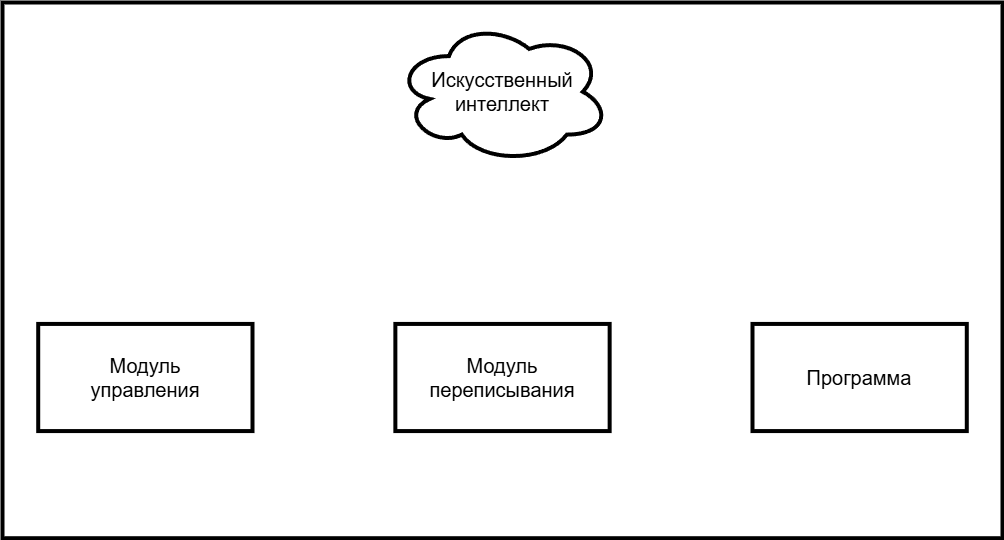
\includegraphics[width=\textwidth]{images/METAMORPHLLM0.png} % Укажите путь к фото 1
        \caption{Этап 1}
        \label{fig:photo_221_1}
    \end{subfigure}% <-- Важный % для удаления пробела
    \hfill % Добавить растяжимое пространство между изображениями
    \begin{subfigure}[b]{0.5\textwidth}
        \centering
        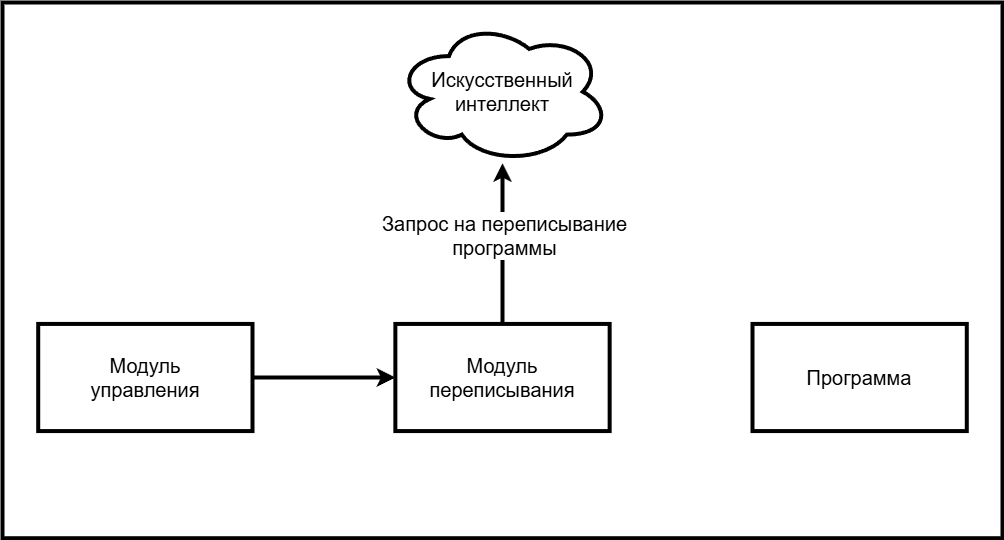
\includegraphics[width=\textwidth]{images/METAMORPHLLM1.png} % Укажите путь к фото 2
        \caption{Этап 2}
        \label{fig:photo_221_2}
    \end{subfigure}

    \vspace{\baselineskip} % Добавить вертикальный отступ между строками

    % --- Вторая строка (2 изображения) ---
    \begin{subfigure}[b]{0.5\textwidth}
        \centering
        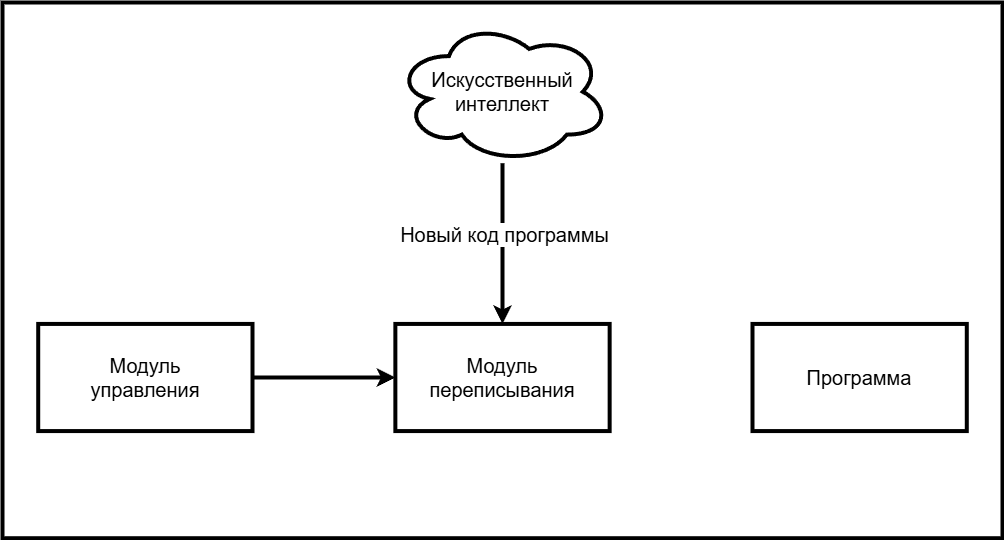
\includegraphics[width=\textwidth]{images/METAMORPHLLM2.png} % Укажите путь к фото 3
        \caption{Этап 3}
        \label{fig:photo_221_3}
    \end{subfigure}% <-- Важный %
    \hfill % Растянуть пространство
    \begin{subfigure}[b]{0.5\textwidth}
        \centering
        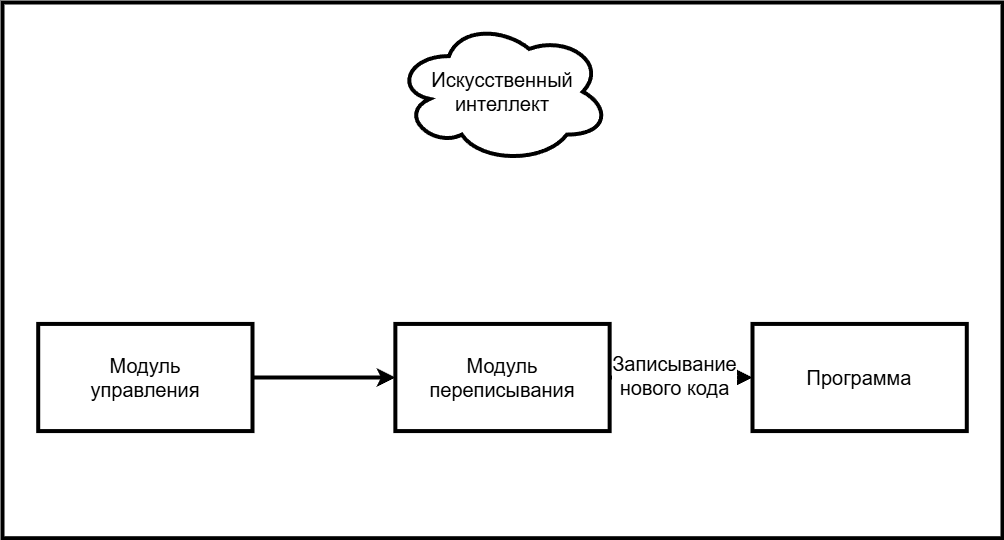
\includegraphics[width=\textwidth]{images/METAMORPHLLM3.png} % Укажите путь к фото 4
        \caption{Этап 4}
        \label{fig:photo_221_4}
    \end{subfigure}

    \vspace{\baselineskip} % Добавить вертикальный отступ между строками

    % --- Третья строка (1 изображение) ---
    % Так как \centering уже есть для всей figure, subfigure будет по центру
    \begin{subfigure}[b]{0.5\textwidth} % Можно сделать шире, если нужно, например 0.5\textwidth
        \centering
        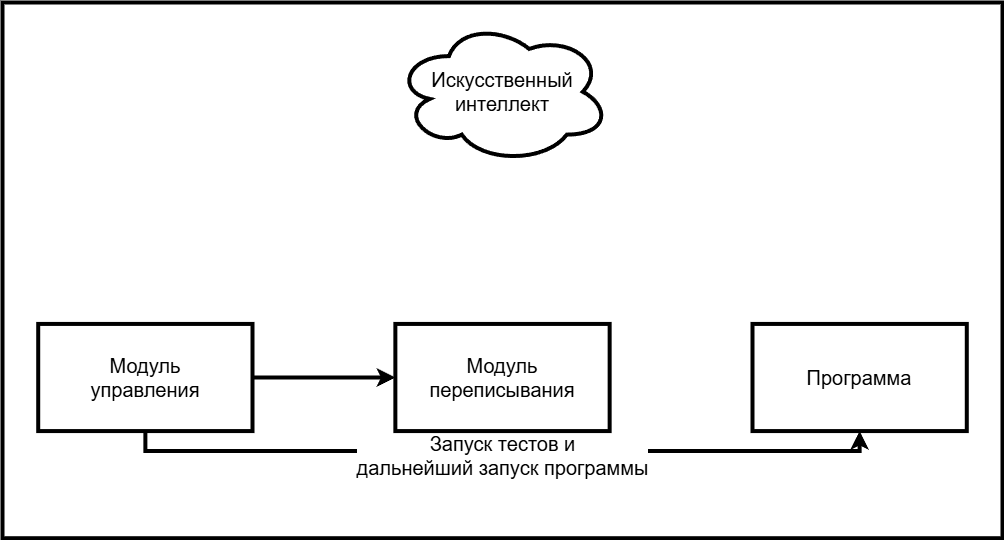
\includegraphics[width=\textwidth]{images/METAMORPHLLM5.png} % Укажите путь к фото 5
        \caption{Этап 5}
        \label{fig:photo_221_5}
    \end{subfigure}

    % --- Общая подпись ко всей группе ---
    \caption{Общая схема работы инструментария.}
    \label{fig:my_five_photos_221} % Метка для ссылки на всю группу

\end{figure*} % Закончить окружение figure

Пользовательский интерфейс реализован в виде CLI-приложения. Этот компонент отвечает за парсинг аргументов командной строки, таких как путь к входному файлу, путь для сохранения результата и выбор используемого API нейронной сети. После валидации входных данных и выбора API, CLI создает экземпляр переписчика из пакета \texttt{internal/rewriter} и вызывает его методы для выполнения основной задачи.

Типичный сценарий работы инструментария выглядит следующим образом: пользователь запускает CLI, указывая исходный файл, желаемый выходной файл и используемый API LLM. Приложение парсит аргументы, создает соответствующий объект переписчика. Переписчик читает исходный файл, формирует и отправляет запрос, включая код и промп, к API выбранной нейронной сети. Получив ответ с модифицированным кодом, переписчик сохраняет результат в указанный выходной файл.

После записи модифицированного кода в файл, проводится замер метрик с выводом результатов в командную строку

Такая архитектура обладает рядом преимуществ. Четкое разделение логики CLI и ядра переписывания упрощает поддержку и тестирование. Добавление поддержки новых LLM API или даже новых техник метаморфизма путем изменения логики формирования промптов требует модификации только внутреннего пакета \texttt{internal/rewriter}, не затрагивая пользовательский интерфейс. Это обеспечивает хорошую расширяемость инструментария.

Оценка качества сгенерированного метаморфического кода проводится на отдельном этапе с использованием метрик функциональной эквивалентности ($FE$), изменения количества строк кода ($LOC_{fin}$), цикломатической сложности ($CC_{fin}$) \cite{McCabe76Complexity} и когнитивной сложности ($CogC_{fin}$) \cite{SonarSourceCogC}, что позволяет количественно измерить как корректность преобразований, так и достигнутый уровень обфускации.
    \section{Метрики оценки}

Для объективной оценки результатов работы разработанного инструментария и сравнения эффективности различных подходов к автоматическому метаморфизму кода недостаточно просто констатировать факт его изменения. Необходимо ввести количественные показатели, которые позволили бы измерить как сохранение исходной функциональности, так и достигнутый уровень усложнения и запутывания кода. Поэтому в данном исследовании был использован набор конкретных метрик, описанных ниже.

Ключевой метрикой является функциональная эквивалентность ($FE$), определяющая степень сохранения семантики программы после метаморфических преобразований. Поскольку основной принцип метаморфизма – изменение формы без изменения содержания, проверка $FE$ является обязательным шагом валидации. В данной работе $FE$ определяется как процент успешно пройденных тестов из заранее подготовленного набора, охватывающего основные сценарии использования модифицируемого кода:
\begin{equation}
FE = \frac{\text{Количество пройденных тестов}}{\text{Общее количество тестов}} \times 100\%
\end{equation}
Идеальным результатом является $FE = 100\%$, любое существенное отклонение свидетельствует о внесении семантических ошибок нейронной сетью в процессе генерации кода.

Для оценки изменения объема кода используется метрика количества строк кода ($LOC$). Хотя $LOC$ является относительно поверхностным показателем, он приобретает значение в контексте техники вставки \enquote{мертвого} кода, которая напрямую подразумевает добавление новых строк. Измеряется абсолютное изменение $\Delta LOC$ и относительное изменение $LOC_{fin}$:
\begin{equation}
\Delta LOC = LOC_{\text{metamorphic}} - LOC_{\text{original}}
\end{equation}
\begin{equation}
LOC_{fin} = \frac{\Delta LOC}{LOC_{\text{original}}} \times 100\%
\end{equation}
Значительный рост $LOC_{fin}$ ожидаем при вставке кода, однако интерпретировать его следует в комплексе с другими метриками сложности.

Для количественной оценки структурной сложности программы применяется цикломатическая сложность ($CC$), предложенная Маккейбом \cite{McCabe76Complexity}. Данная метрика основана на анализе графа потока управления и определяет количество линейно независимых путей в коде, что коррелирует с трудоемкостью тестирования. Формула расчета: 
\begin{equation}
CC = E - N + 2P
\end{equation}
где $E$ — количество рёбер в графе, $N$ — количество узлов, $P$ — количество связных компонентов. В контексте метаморфизма, особенно при модификации потока управления, ожидается рост $CC$ из-за усложнения управляющих конструкций. Рассчитывается относительное изменение:
\begin{equation}
\Delta CC = CC_{\text{metamorphic}} - CC_{\text{original}}
\end{equation}
\begin{equation}
CC_{fin} = \frac{\Delta CC}{CC_{\text{original}}} \times 100\%
\end{equation}
Положительное значение $CC_{fin}$ свидетельствует об усложнении структуры программы.

Для оценки сложности кода с точки зрения его понимания человеком-разработчиком используется когнитивная сложность ($CogC$). В отличие от $CC$, метрика $CogC$ штрафует за конструкции, прерывающие линейный поток чтения кода (условия, циклы, `goto`, рекурсия) и за их вложенность \cite{SonarSourceCogC}. Обе реализованные техники метаморфизма потенциально увеличивают $CogC$. Измеряется относительное изменение:
\begin{equation}
\Delta CogC = CogC_{\text{metamorphic}} - CogC_{\text{original}}
\end{equation}
\begin{equation}
CogC_{fin} = \frac{\Delta CogC}{CogC_{\text{original}}} \times 100\%
\end{equation}
Рост $CogC_{fin}$ интерпретируется как повышение сложности восприятия и анализа кода человеком.

Совокупность этих четырех метрик ($FE$, $LOC_{fin}$, $CC_{fin}$, $CogC_{fin}$) позволяет получить многогранную картину результатов метаморфизма, сравнивая как корректность преобразований, так и эффективность различных нейронных сетей и техник в задаче обфускации кода.

    \section{Экспериментальная оценка и анализ результатов}

После разработки и реализации инструментария был проведен цикл вычислительных экспериментов для количественной оценки эффективности предложенного подхода и сравнения результатов, достигаемых различными моделями искусственного интеллекта. Экспериментальная установка включала описанный инструментарий, тестовую программу на Go и три нейронные сети на основе архитектуры Трансформер: \texttt{gemini-2.5-flash-preview-04-17}, \texttt{deepseek-chat-v3-0324} и \texttt{gemini-2.0-flash}, доступ к которым осуществлялся через API. Для каждой модели и целевой техники метаморфизма (вставка \enquote{мертвого} кода или модификация потока управления) использовался специализированный промпт, содержащий подробное объяснение техники метаморфизма, пример использования, основные замечания по генерации кода на Go и исходный код, который подлежит модификации. Проверка функциональной эквивалентности $FE$ проводилась отдельно для каждого сгенерированного варианта. В данном разделе анализируются показатели $FE$ и метрики обфускации ($LOC_{fin}$, $CC_{fin}$, $CogC_{fin}$) для успешно скомпилированных модификаций.

Сводные усредненные данные экспериментов представлены в Таблице~\ref{tab:exp_results}.

\begin{table*}[ht!]
\centering
\captionsetup{justification=centering} % Центрирование подписи таблицы
\caption{Медианные значения метрик для различных моделей нейронных сетей и техник метаморфизма}
\label{tab:exp_results}
% Определяем таблицу шириной в \textwidth
% X столбец - растягиваемый с переносом текста, выравнивание по левому краю
% >{\RaggedRight} используется для лучшего вида левого выравнивания в X
% c - центрированный столбец
% @{} убирает пробелы по краям таблицы
\begin{tabularx}{16cm}{@{} >{\RaggedRight}X >{\RaggedRight}Xcccc@{}}
\toprule
\textbf{Модель} & \textbf{Техника} & \textbf{$FE$ (\%)} & \textbf{$LOC_{fin}$ (\%)} & \textbf{$CC_{fin}$ (\%)} & \textbf{$CogC_{fin}$ (\%)} \\
\midrule
\multicolumn{6}{@{}l}{\textit{gemini-2.5-flash-preview-04-17}} \\
\midrule
 & Вставка \enquote{мертвого} кода & 93 & \textbf{612} & \textbf{640} & \textbf{905} \\
 & Модификация потока & \textbf{100} & \textbf{297} & \textbf{167} & \textbf{1121} \\
\midrule
\multicolumn{6}{@{}l}{\textit{deepseek-chat-v3-0324}} \\
\midrule
 & Вставка \enquote{мертвого} кода & 92 & 161 & 284 & 417 \\
 & Модификация потока & 43 & 89 & 90 & 321 \\
\midrule
\multicolumn{6}{@{}l}{\textit{gemini-2.0-flash}} \\
\midrule
 & Вставка \enquote{мертвого} кода & \textbf{100} & 245 & 443 & 619 \\
 & Модификация потока & 53 & 211 & 72 & 702 \\
\bottomrule
\end{tabularx}
\end{table*}

Анализ результатов позволяет сравнить влияние техник метаморфизма и эффективность различных моделей LLM. Техника вставки \enquote{мертвого} кода стабильно обеспечивает высокую функциональную эквивалентность (92-100\%) при значительном увеличении объема кода и существенном росте метрик сложности. Это указывает на способность LLM генерировать семантически нейтральный, но объемный и структурно сложный дополнительный код.

Модификация потока управления демонстрирует иные тенденции. Прирост объема кода значительно ниже, что ожидаемо. Ключевым эффектом является резкое увеличение когнитивной сложности ($CogC_{fin}$ до 1121\%), подтверждая гипотезу о том, что данная техника наиболее эффективно затрудняет понимание кода человеком \cite{SonarSourceCogC}. Однако сохранение функциональной эквивалентности ($FE$) при этой технике оказалось серьезной проблемой для моделей \texttt{deepseek-chat-v3-0324} (43\%) и \texttt{gemini-2.0-flash} (53\%). Лишь модель \texttt{gemini-2.5-flash-preview-04-17} смогла обеспечить 100\% $FE$ при модификации потока, показав при этом максимальный прирост $CogC_{fin}$. Низкий прирост цикломатической сложности у некоторых моделей при модификации потока может свидетельствовать о генерации конструкций, запутанных для человека, но не обязательно увеличивающих число путей выполнения так же сильно, как вставка сложного \enquote{мертвого} кода.

Сравнение моделей LLM выявило различные профили эффективности. Модель \texttt{gemini-2.5-flash-preview-04-17} проявила себя как наиболее эффективная, обеспечивая максимальные показатели усложнения, особенно при вставке кода, и являясь единственной моделью, сохранившей 100\% $FE$ при модификации потока. Модель \texttt{deepseek-chat-v3-0324} показала наименее выраженные результаты, с наименьшим усложнением и крайне низкой $FE$ при модификации потока. Модель \texttt{gemini-2.0-flash} продемонстрировала компромиссный результат: идеальная $FE$ при вставке кода с хорошим усложнением, но низкая $FE$ при модификации потока, несмотря на высокий прирост $CogC_{fin}$. Выбор оптимальной модели зависит от приоритетов: максимальная обфускация или гарантированная функциональность.

В целом, эксперименты подтвердили эффективность автоматизированного метаморфизма с использованием LLM для кода Go. Достигнут значительный прирост метрик сложности, что демонстрирует потенциал подхода для усложнения анализа. Однако выявлены ключевые проблемы: нестабильность сохранения функциональной эквивалентности, особенно при модификации потока управления, что подчеркивает необходимость тщательного тестирования. Текущие метрики дают лишь косвенную оценку стойкости к реверс-инжинирингу, и требуется разработка более точных методов оценки. Зависимость от качества промптов и вариативность ответов LLM также требуют дальнейшего изучения.

Анализ метрик обфускации ($LOC_{fin}$, $CC_{fin}$, $CogC_{fin}$) количественно подтвердил, что применение разработанного подхода приводит к значительному усложнению программного кода. Особенно впечатляющие результаты показала модель \texttt{gemini-2.5-flash-preview-04-17}, продемонстрировав как наилучшую функциональную эквивалентность при модификации потока управления (100\%), так и максимальные показатели усложнения по метрикам когнитивной сложности. Относительный прирост цикломатической и когнитивной сложности свидетельствует о потенциале метода для затруднения анализа и понимания кода как автоматизированными средствами, так и человеком.

    \section{Заключение и Будущие направления}

В ходе выполнения данной работы был успешно разработан и апробирован инструментарий для автоматизации метаморфизма кода на языке Go, использующий возможности современных больших языковых моделей. Основной целью являлось исследование применимости нейронных сетей для генерации семантически эквивалентных, но структурно измененных вариантов кода, реализующих техники вставки \enquote{мертвого} кода и модификации потока управления.

Ключевым результатом работы является демонстрация принципиальной возможности автоматизации метаморфизма с помощью LLM. Созданный прототип инструментария с модульной архитектурой способен итеративно модифицировать Go-код, делегируя генерацию преобразований внешним API нейронных сетей. Проведенные эксперименты с тремя различными моделями LLM показали, что они способны генерировать код, который в большинстве случаев успешно компилируется и сохраняет исходную функциональность, особенно при использовании техники вставки \enquote{мертвого} кода.

Анализ метрик обфускации ($LOC_{fin}$, $CC_{fin}$, $CogC_{fin}$) количественно подтвердил, что применение разработанного подхода приводит к значительному усложнению программного кода. Особенно впечатляющие результаты показала модель gemini-2.5-flash-preview-04-17, продемонстрировав как наилучшую функциональную эквивалентность при модификации потока управления (100\%), так и максимальные показатели усложнения по метрикам когнитивной сложности. Относительный прирост цикломатической и когнитивной сложности свидетельствует о потенциале метода для затруднения анализа и понимания кода как автоматизированными средствами, так и человеком.

Вклад данной работы заключается в предложении нового подхода к автоматизации метаморфизма, основанного на использовании LLM и применимого к исходному коду Go. Проведенное сравнение различных LLM в контексте этой специфической задачи также представляет практический и научный интерес.

Несмотря на достигнутые результаты, выявленные ограничения определяют направления для дальнейших исследований. Основными вызовами остаются обеспечение стопроцентной гарантии сохранения функциональной эквивалентности при сложных преобразованиях потока управления, а также разработка более точных и комплексных метрик для оценки реальной стойкости обфусцированного кода к инструментам реверс-инжиниринга.

Перспективные направления дальнейших исследований включают:
\begin{itemize}
    \item Расширение набора реализуемых техник метаморфизма.
    \item Исследование и оптимизация методов взаимодействия с LLM, в том числе fine-tuning специализированных моделей для задач преобразования кода.
    \item Интеграция механизмов обратной связи для адаптивного управления процессом метаморфизма.
    \item Разработка более совершенных метрик оценки стойкости обфускации к современным инструментам анализа.
    \item Тестирование инструментария на более крупных и сложных реальных проектах на Go для оценки практической применимости и масштабируемости.
\end{itemize}
Развитие предложенного подхода имеет потенциал для создания нового поколения интеллектуальных инструментов защиты программного обеспечения.

}

% Название статьи
\newcommand*{\Title}{%
    Автоматизация метаморфизма кода Go с использованием больших языковых моделей%
}

% Название статьи на английском
\newcommand*{\TitleEN}{%
    Automating Go Code Metamorphism Using Large Language Models%
}

% Список авторов работы
\newcommand*{\Authors}{%
    Д.~К.~Мурадян, О.~В.~Цветков%
}

% Список авторов работы на английском
\newcommand*{\AuthorsEN}{%
    David Muradyan, Oleg Tsvetkov%
}

% Информация об авторах
\newcommand*{\AuthorsInfo}{%
    \thanks{Давид Каренович Мурадян, МГУ им. М.В.~Ломоносова, (email: itzkhaotic1@gmail.com).}%
    \thanks{Олег Вячеславович Цветков, РТУ МИРЭА, (email: oleg@tsv.one).}%
}

% Дата, когда статья была отправлена в редакцию
\newcommand*{\DateOfSubmission}{%
    1 мая 2025%
}

% Укажите информацию о гранте, в рамках которого выполняется работа
\newcommand*{\Grant}{%
    % Исследование выполнено частично при финансовой поддержке ???? в рамках научного проекта ?????.%
}

% Аннотация
\newcommand*{\Abstract}{%
     Метаморфизм кода является мощной техникой защиты программного обеспечения от реверс-инжиниринга, однако его ручная реализация крайне трудоемка. В данной работе представлен инструментарий для автоматизации процесса метаморфизма кода на языке Go с использованием больших языковых моделей. Инструментарий реализует модульную архитектуру и применяет две ключевые техники: вставку \enquote{мертвого} кода и модификацию потока управления, делегируя генерацию преобразований внешним LLM. Проведена экспериментальная оценка с использованием трех современных больших языковых моделей (gemini-2.5-flash-preview-04-17, deepseek-chat-v3-0324, gemini-2.0-flash). Эффективность оценивалась по метрикам функциональной эквивалентности, изменения количества строк кода, цикломатической и когнитивной сложностей. Результаты демонстрируют возможность автоматизации метаморфизма с помощью LLM, значительное усложнение кода по метрикам CC и CogC, но выявляют проблемы со стабильностью сохранения функциональности при модификации потока управления у некоторых моделей. Работа показывает перспективность использования LLM для задач обфускации кода, но подчеркивает необходимость дальнейших исследований для повышения надежности и оценки реальной стойкости кода.
}

% Аннотация на английском
\newcommand*{\AbstractEN}{%
    Code metamorphism is a powerful technique for protecting software from reverse engineering, but its manual implementation is extremely labor-intensive. This paper presents a toolkit for automating the code metamorphism process for the Go language using large language models. The toolkit implements a modular architecture and applies two key techniques: dead code insertion and control flow modification, delegating the generation of transformations to external LLMs. An experimental evaluation was conducted using three modern LLMs (gemini-2.5-flash-preview-04-17, deepseek-chat-v3-0324, gemini-2.0-flash). Effectiveness was assessed using metrics of functional equivalence, change in lines of code, cyclomatic complexity, and cognitive complexity. The results demonstrate the feasibility of automating metamorphism with LLMs, a significant increase in code complexity according to CC and CogC metrics, but reveal issues with the stability of maintaining functional equivalence during control flow modification for some models. The work shows the promise of using LLMs for code obfuscation tasks but highlights the need for further research to improve reliability and assess the real-world resilience of the code.
}

% Ключевые слова
\newcommand*{\Keywords}{%
    метаморфизм кода, обфускация кода, большие языковые модели, LLM, Go, автоматизация, защита программного обеспечения, сложность кода, цикломатическая сложность, когнитивная сложность%
}

% Ключевые слова на английском
\newcommand*{\KeywordsEN}{%
    сode metamorphism, code obfuscation, large language models, LLM, Go, automation, software protection, code complexity, cyclomatic complexity, cognitive complexity%
}

%%%% Эти параметры нужно задать после принятия статьи к опубликованию
%%%% Редакция пришлёт информацию какие значения параметров нужно установить
%%%%%% Том
\newcommand*{\Vol}{?} % Будет заполнено редакцией
%%%%%% Номер
\newcommand*{\Number}{?} % Будет заполнено редакцией
%%%%%% Год издания
\newcommand*{\Year}{\the\year}
%%%%%% Номер первой страницы
\newcommand*{\FirstPageNumber}{1} % Будет уточнено редакцией
